\documentclass[11pt,aspectratio=43]{beamer}

\usetheme[progressbar=frametitle]{Madrid} % Frankfurt default
%\usepackage{appendixnumberbeamer}

\usepackage{booktabs}
%\usepackage[scale=2]{ccicons}

\usepackage{pgfplots}
\usepgfplotslibrary{dateplot}

\usepackage{xspace}
\newcommand{\themename}{\textbf{\textsc{metropolis}}\xspace}

\usepackage{xcolor}

\usepackage{physics}
\usepackage{amsmath}
\usepackage{slashed}
\usepackage{dsfont}
%\usepackage[dvipsnames]{xcolor}
\usepackage{bm}
\usepackage{makecell}
% Justify text (package and function)
% \apptocmd{command}{code}{success}{failure}
%\apptocmd{\frame}{}{\justifying}{} 
% Justify text in \item
\newcommand{\itemj}{\item \justifying}
\useinnertheme{circles}
% If...else package
\usepackage{ifthen}

\usepackage[english]{babel}
%\usepackage[latin1]{inputenc}
\usepackage[T1]{fontenc}
\usepackage{caption}
\usepackage{multimedia}
\usepackage{hyperref}
\usepackage{setspace}
\usepackage{subfigure}
\usepackage{ragged2e}
\usepackage{dirtytalk}
% Bibliography packages
%\usepackage[style=authoryear,backend=bibtex]{biblatex}
%\setbeamertemplate{bibliography item}{\insertbiblabel} 
%\addbibresource{mb.bib}
\usepackage[absolute,overlay]{textpos}
\usepackage[export]{adjustbox} % valign to align equations and figures
\usepackage{etoolbox}
\usepackage{bbold}
\usepackage{tikz} %progress bar
\usepackage{cancel}
\usetikzlibrary{arrows,shapes}
\usepackage[skins,theorems]{tcolorbox}
\tcbset{highlight math style={enhanced,
  colframe=red,colback=white,arc=0pt,boxrule=1pt}}
\usepackage{csquotes}
  
%\usepackage{footbib}
% Bibliography packages
%\usepackage{bibentry}
\usepackage[style=authoryear,backend=biber]{biblatex}
%\setbeamertemplate{bibliography item}{\insertbiblabel} 
\addbibresource{mb.bib}
\definecolor{mygreencite}{rgb}{0, .5, 0.}
\DeclareCiteCommand{\cite}
    {\footnotesize \color{mygreencite}[\usebibmacro{prenote}}%
    {\usebibmacro{citeindex}%
    \usebibmacro{cite}}
    {\multicitedelim}
    {\usebibmacro{postnote}]
}

%Graphics and Videos
\usepackage{graphicx} %The mode "LaTeX => PDF" allows the following formats: .jpg  .png  .pdf  .mps
\graphicspath{{./Plots/}} %Where the figures folder is located
\usepackage{media9,xcolor}
\addmediapath{./Movies/}
% Set figure number when included
%\setbeamertemplate{caption}[numbered]

\usepackage{amssymb}% http://ctan.org/pkg/amssymb
\usepackage{pifont}% http://ctan.org/pkg/pifont

\definecolor{myblue}{rgb}{0, .44, 1.}
\definecolor{myviolet1}{rgb}{0., .22, 1.}
\definecolor{myviolet2}{rgb}{.7, 0.5, 1.}

\usecolortheme[named=myblue]{structure}
%\setbeamercovered{dynamic}

% Set theme palette colors
\setbeamercolor{palette primary}{bg=myblue,fg=white}
\setbeamercolor{palette secondary}{bg=myviolet1,fg=white}
\setbeamercolor{palette tertiary}{bg=myviolet2,fg=white}
\setbeamercolor{palette quaternary}{bg=myblue,fg=white}
% strucure means itemize, enumerate, etc
\setbeamercolor{structure}{fg=myblue}

% Set bibliography colors
\setbeamercolor{bibliography item}{fg=myblue}
\setbeamercolor{bibliography entry author}{fg=black}
\setbeamercolor{bibliography entry title}{fg=black}
\setbeamercolor{bibliography entry location}{fg=black}
\setbeamercolor{bibliography entry note}{fg=black}
% Replaces book icon in bibliography with enumeration
%\setbeamertemplate{bibliography item}{[\theenumiv]}

\mode<presentation>{}
\setbeamertemplate{frametitle continuation}{}

\setbeamertemplate{navigation symbols}{}

% Header with navigation bar
\setbeamertemplate{headline}
{
	%\usebeamerfont{size=\small}
	\setbeamerfont{section in head/foot}{size=\normalsize}
	\leavevmode
	\hbox{
	\begin{beamercolorbox}[wd=\paperwidth,ht=6ex,dp=3ex]{palette quaternary}
		%\insertsectionnavigationhorizontal{\paperwidth}{}{\hskip0pt plus1filll} %align section names on the right
		\insertsectionnavigationhorizontal{\paperwidth}{\hskip0pt plus1fill}{\hskip0pt plus1fill} %center section names
	\end{beamercolorbox} 
	}
}

% Footer with custom caption
\setbeamertemplate{footline}
{
	\leavevmode
	\hbox{
	\begin{beamercolorbox}[wd=.23\paperwidth,ht=2.6ex,dp=1ex,center]{palette tertiary}
		\usebeamerfont{author in head/foot}\insertshortauthor\hspace*{1ex}
	\end{beamercolorbox}
	\begin{beamercolorbox}[wd=.53\paperwidth,ht=2.6ex,dp=1ex,center]{palette primary}
		\usebeamerfont{title in head/foot}\insertshorttitle
	\end{beamercolorbox}
	\begin{beamercolorbox}[wd=.23\paperwidth,ht=2.6ex,dp=1ex,center]{palette secondary}
		%\usebeamerfont{date in head/foot}\insertshortdate{}\hspace*{2em}
		\insertframenumber{} / \inserttotalframenumber
	\end{beamercolorbox}}
	\vskip 0pt
}

\title[Short Title]{Long Title}
%\subtitle{}
% \date{\today}
\date[17/09/1997]{
\begin{columns}
\column{0.1\linewidth}
\column{0.2\linewidth}
% Logo of the conference
\centering 
\includegraphics[width=1cm]{DUCK_2}
\column{0.6\linewidth}
\centering Name of the conference \\ September 17th, 1997
\end{columns}
\vspace{\baselineskip}
Relying on: \textit{Dalla Brida, Giusti, Harris, Pepe, PLB 816 (2021) 136191}
}
\author[Matteo Saccardi]{ {\Large{Matteo~Saccardi}} \texorpdfstring{\\}{} In collaboration with Some~One, El~Se}\relax
\institute[]{
\begin{columns}
\column{0.5\linewidth}
\centering 
\includegraphics[width=2.5cm]{LOGO_UNIMIB}
\column{0.5\linewidth}
\centering 
\includegraphics[width=5cm]{LOGO_INFN.pdf}
\end{columns}
}\relax
%\titlegraphic{\hfill\includegraphics[height=1.5cm]{logo.jpg}}
%\logo{\hfill\includegraphics[height=1.5cm]{logo.jpg}}


%\usetheme{Madrid}
%\usetheme{AnnArbor}
%\useoutertheme[right]{sidebar}

%\usebackgroundtemplate{%
%\tikz\node[opacity=0.1] {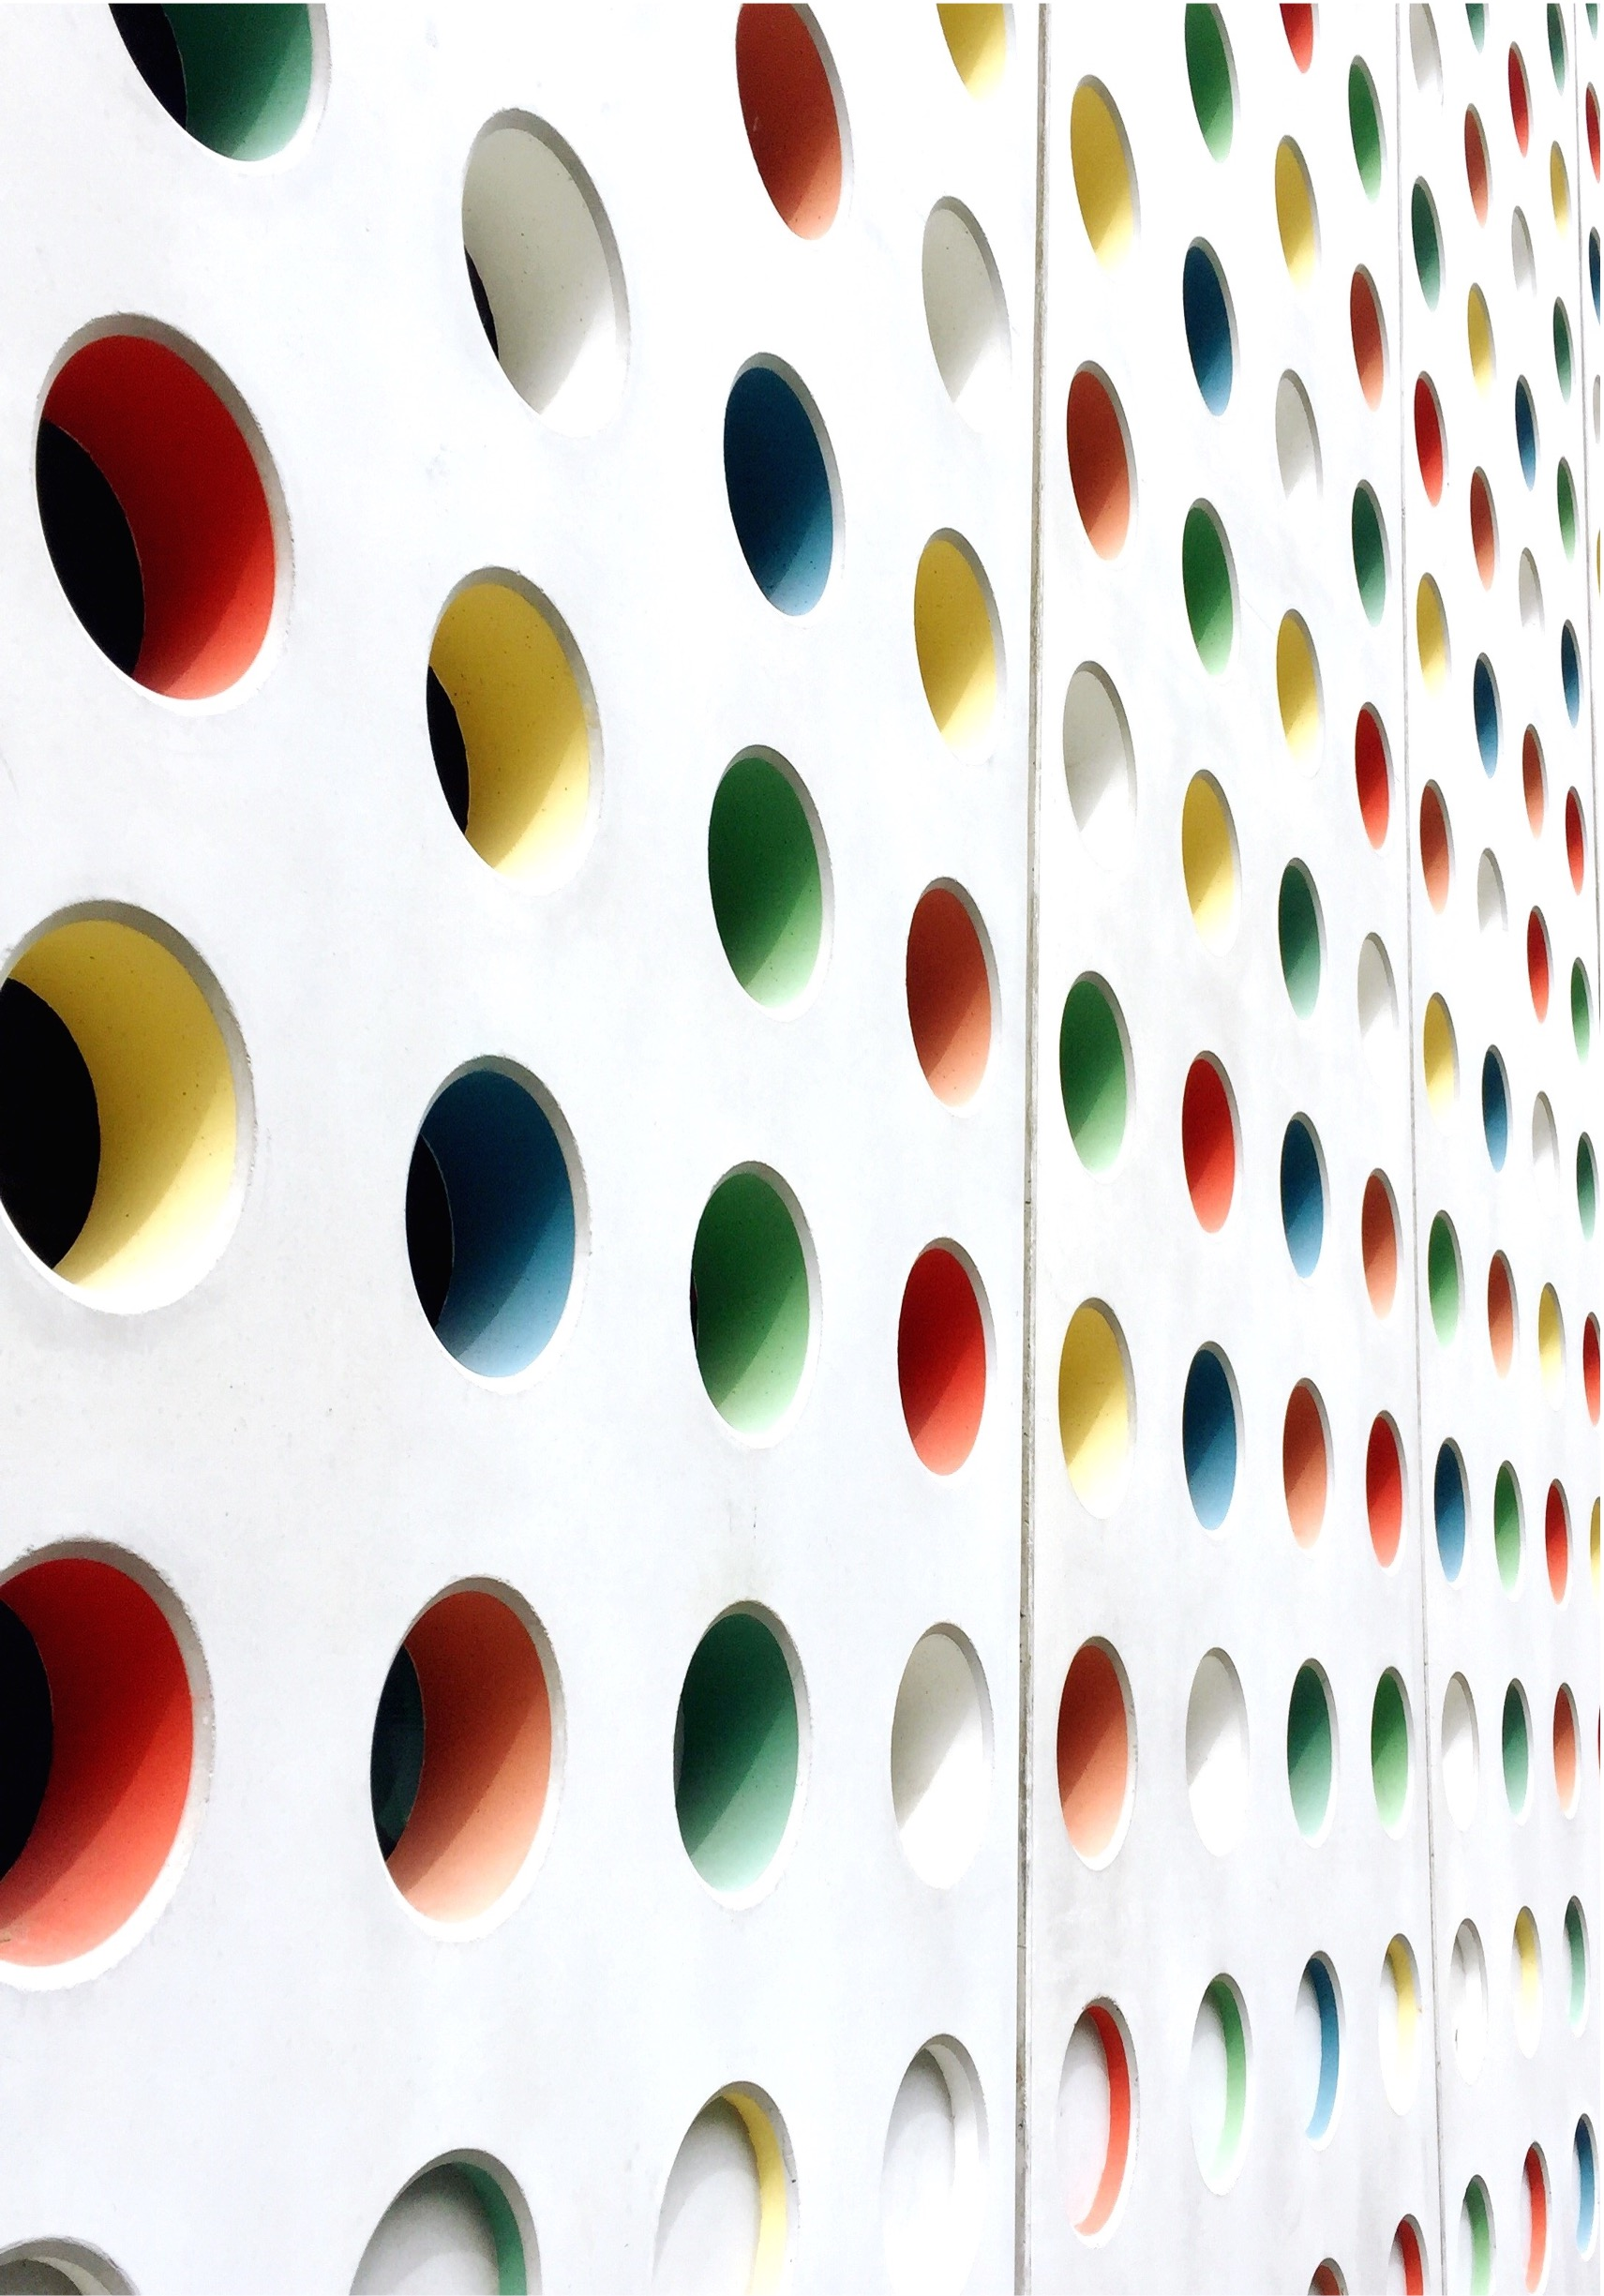
\includegraphics[height=\paperheight,width=\paperwidth]{background}};}
\pgfplotsset{compat=1.18}

\begin{document}
{
\usebackgroundtemplate{
\tikz\node[opacity=0.25] {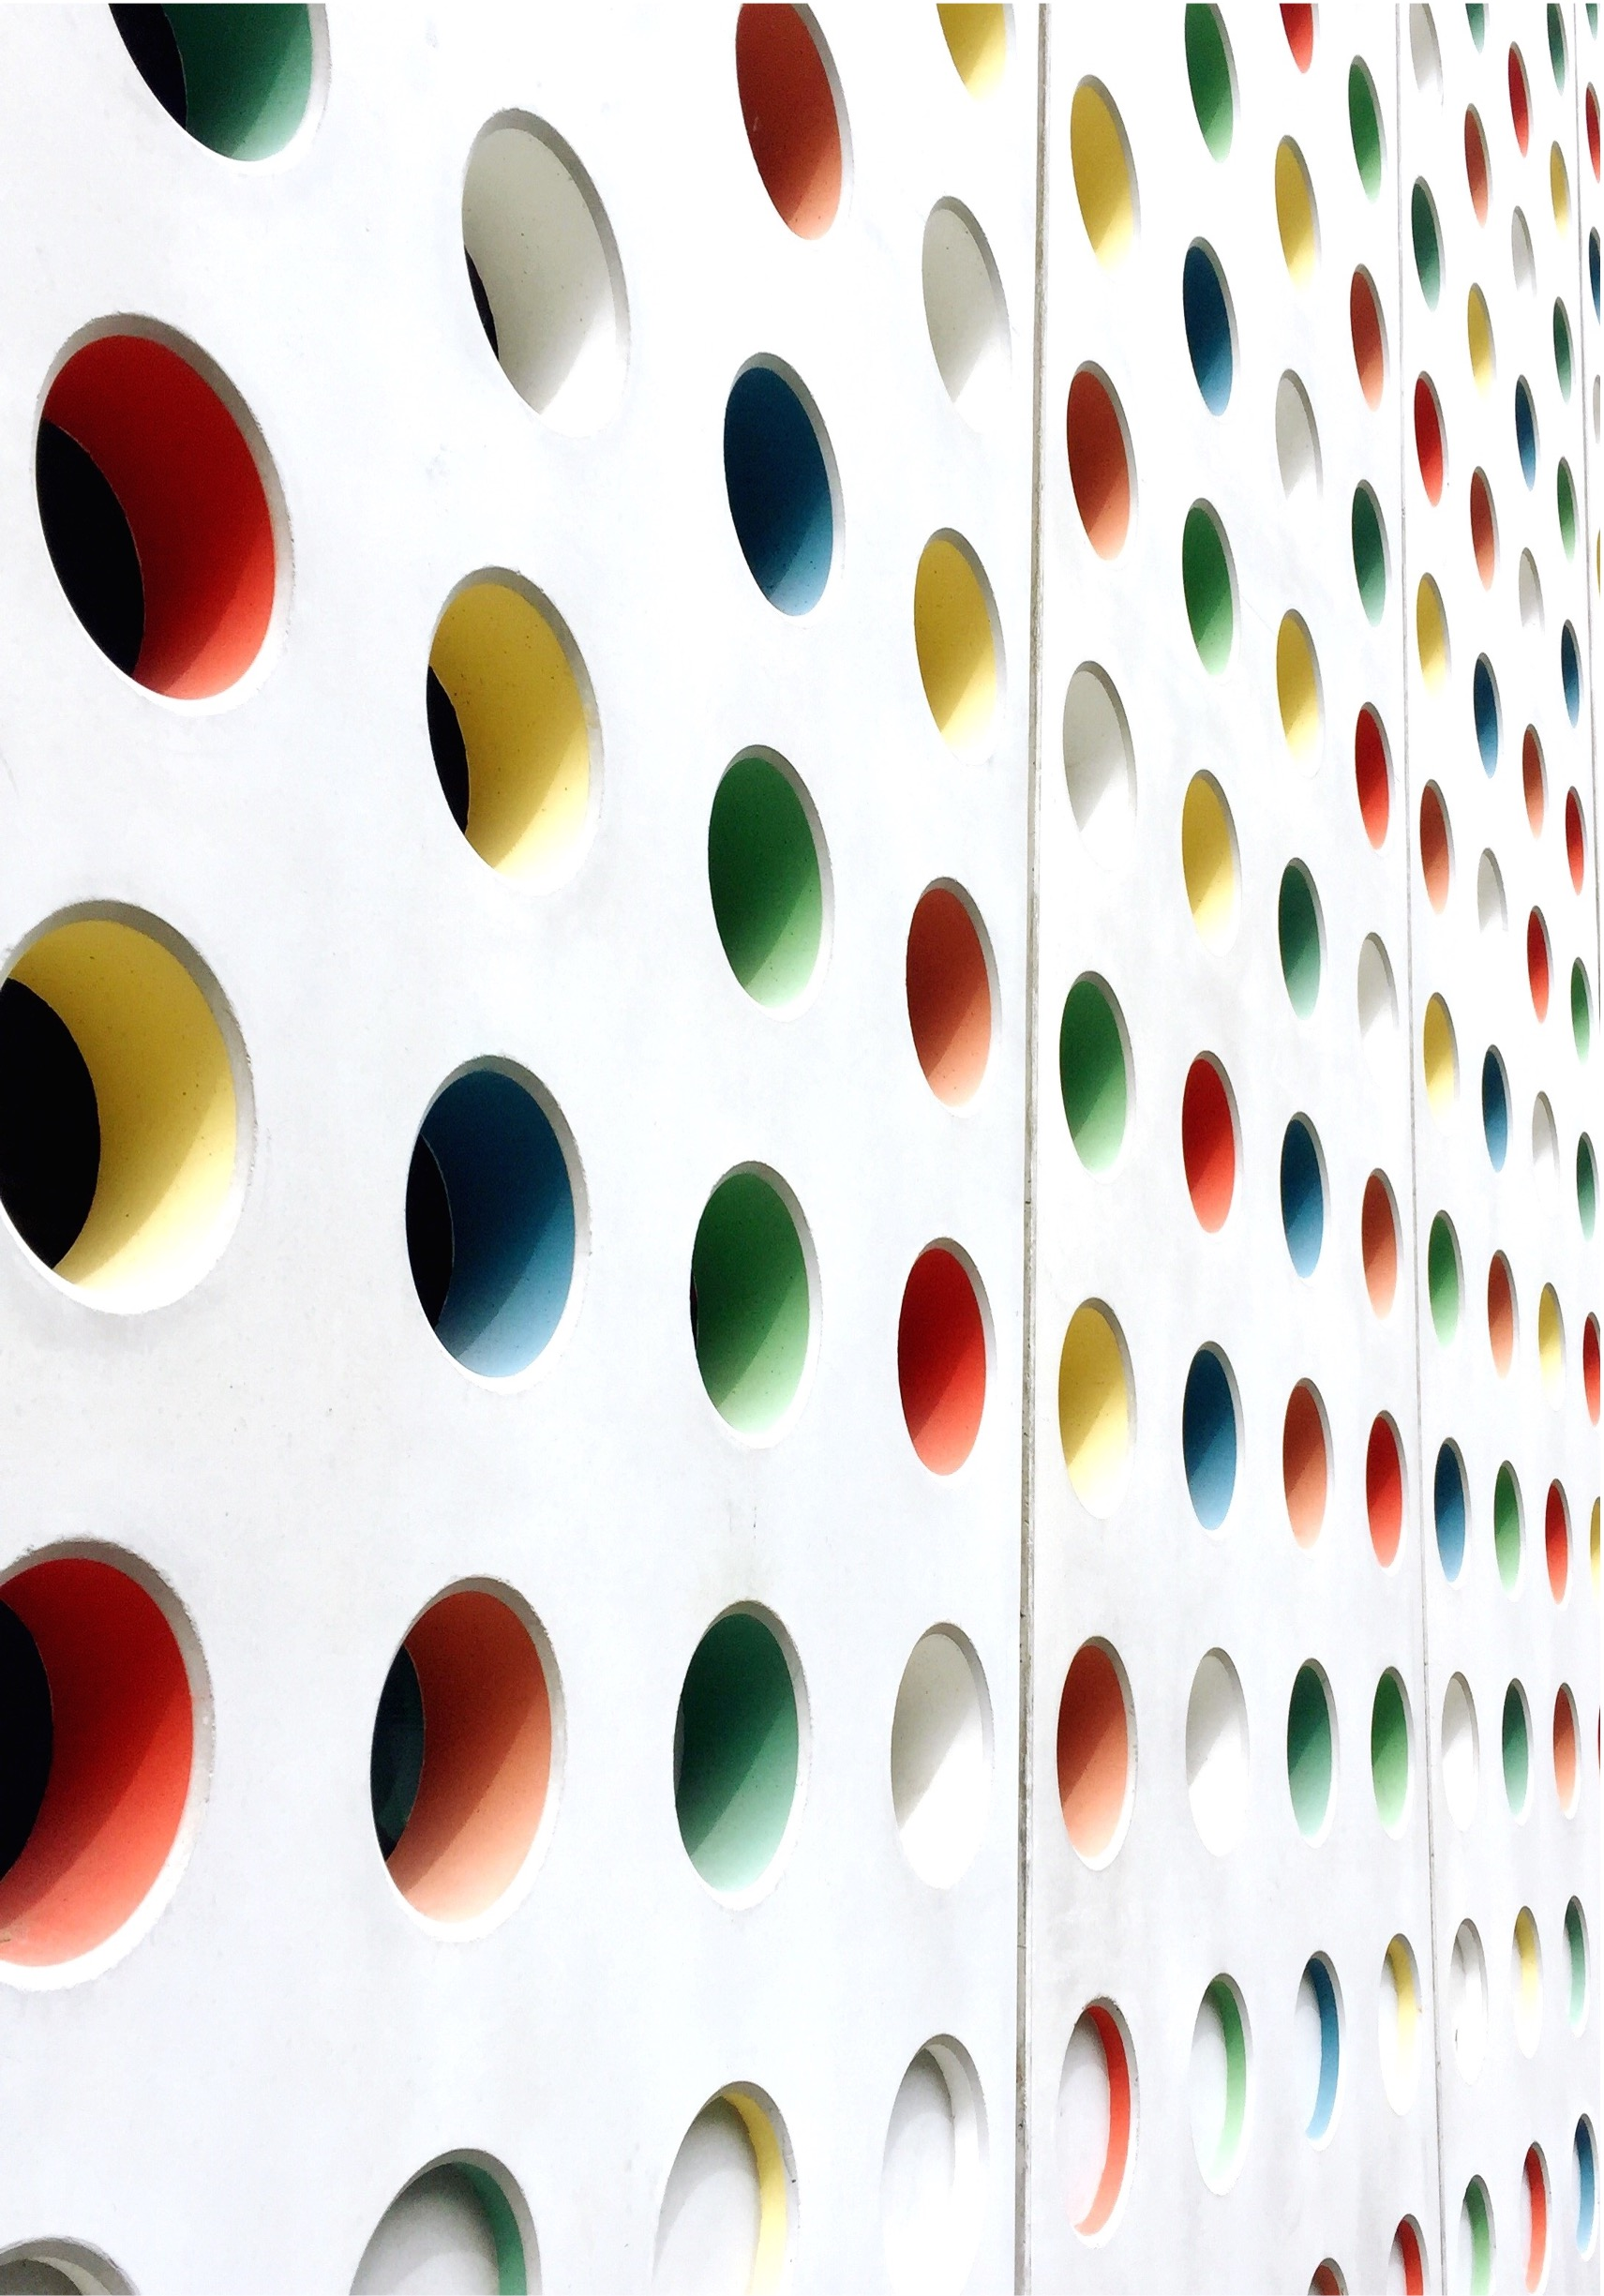
\includegraphics[width=\paperwidth]{background}};}
\begin{frame}[plain,noframenumbering]
\maketitle
\end{frame}
}

%\begin{frame}{}
%  \setbeamertemplate{section in toc}[sections numbered]
%  \tableofcontents[hideallsubsections]
%\end{frame}

\section{Introduction and Motivations}

\begin{frame}{}

\begin{itemize}
    \item The analytical integration of fermionic degrees of freedom
    \begin{equation*}
        \int \mathcal{D} U e^{-S_G[U]} \int \mathcal{D} \psi \mathcal{D} \bar\psi e^{-\bar\psi D[U] \psi} = \int \mathcal{D} U e^{-S_G[U]} \det D[U]
    \end{equation*}
    leads to an effective bosonic theory with action
    \begin{equation*}
        S^{eff}[U] = \underbrace{S_G[U]}_\text{\large{local}} + \underbrace{S_F^{eff}[U]}_\text{\large{global}}, \qquad S_F^{eff}[U] = - \ln{\det D[U]}
    \end{equation*}
    \item Aim: factorize $\det D[U]$
    \item Here: factorization via an overlapping $4d$ domain decomposition \cite{GIUSTI2022137103}
\end{itemize}
\end{frame}

\section{Problem Setting}


\begin{frame}{}
\centering
\begin{equation*}
	i \hbar \partial_t \psi = H \psi, \quad H = -\frac{\hbar^2}{2m}\nabla^2 + V(x)
\end{equation*}
\end{frame}

\section{A Solution}


\begin{frame}{}
\centering
\begin{equation*}
	\left( i \slashed{\partial} - m \right) \psi = 0
\end{equation*}
\end{frame}


\section{Outlook}


\begin{frame}{}
\begin{itemize}
    \item \textbf{Multi-level}: local updates and averages \vspace{\baselineskip}
    \item \textbf{Master-field}: fully factorized molecular-dynamics evolution \vspace{\baselineskip}
    \item \textbf{Parallelization} on heterogeneous architectures \vspace{\baselineskip}
\end{itemize}
\onslide<2->{
\vspace{\baselineskip}
\begin{center}
    \textbf {\color{myblue} \Large Thank you for your attention!}
\end{center}
}
\end{frame}

%

\begin{frame}<0>[plain,noframenumbering]
\centering \textbf { \Large \color{myblue} \emph{Backup slides}}
\end{frame}

\begin{frame}[plain,noframenumbering]
\begin{columns}
\column{0.5\linewidth}
\centering \textbf { \Large \color{myblue} \emph{Backup slides}}
\column{0.5\linewidth}
\centering 
\includegraphics[width=4cm]{DUCK_1}
\end{columns}
\end{frame}

\begin{frame}<0>[plain,noframenumbering]
\begin{columns}
\column{0.5\linewidth}
\centering \textbf { \Large \color{myblue} \emph{Backup slides}}
\column{0.5\linewidth}
\centering 
\includegraphics[width=3cm]{DUCK_2}
\end{columns}
\end{frame}

\appendix

\begin{frame}[plain,noframenumbering]{LU decomposition of a $2\times 2$ block matrix}
  \begin{gather*}
      M = \begin{pmatrix} A & B \\ C & D \end{pmatrix}
      = \begin{pmatrix} I & BD^{-1} \\ 0 & I \end{pmatrix}
      \begin{pmatrix} S_A & 0 \\ C & D \end{pmatrix}, S_A = A-B D^{-1} C \\
      \det M = \det D \det S_A \\
      M^{-1} = \begin{pmatrix} S_A^{-1} & -S_A^{-1} B D^{-1} \\ -D^{-1}C S_A^{-1} & D^{-1}+D^{-1} C S_A^{-1} B D^{-1} \end{pmatrix} \\
      \det \begin{pmatrix} A & \mathcal{B} \\ \mathcal{C} & D \end{pmatrix} = \det A \det D \det \begin{pmatrix} 1 & \mathcal{A}^{-1} \mathcal{B} \\ \mathcal{D}^{-1} \mathcal{C} & 1 \end{pmatrix} \\
      \mathcal{A}^{-1} = P_1 A^{-1} P_1, \mathcal{B} = P_1 B P_2, \mathcal{C} = P_2 C P_1, \mathcal{D}^{-1} = P_2 D^{-1} P_2
  \end{gather*}
\end{frame}

%\begin{frame}[allowframebreaks]{References}

%  \bibliography{main}
%  \bibliographystyle{abbrv}

%\end{frame}

\end{document}
